\documentclass{Teunw}
\usepackage{graphicx}
\usepackage{float}
\usepackage[dutch]{babel} % Used for dutch naming on image caption
\title{Release Plan Groep 5}
\author{Teun Willems, Jules Kreutzer}

\begin{document}
	\maketitle
	
	\tableofcontents
	\pagenumbering{gobble}
	
	\chapter{Version Control}
	Door middel van version control kunnen meerdere ontwikkelaars aan dezelfde software werken.
	Tijdens JEA6 zal Git (GitHub) gebruikt worden voor version control. Er is hiervoor gekozen omdat hiermee reeds de meeste ervaring is opgedaan.
	
	\begin{figure}[H]
			\includegraphics[width=0.50\textwidth]{images/configuredBranches.png}
			\caption{Overzicht van default branch en protected branches}
			\label{fig:ConfiguredBranches}
	\end{figure}
	
	\section{Branches}
	Voor de repository waar de code van het vak JEA6 wordt bijgehouden, zijn verschillende branches aangemaakt. Wat het nu is van deze verschillende branches, staat in de volgende alinea's uitgelegd.
	
	\subsection{Master}
	De code die beschikbaar is in de master-branch, is de code van de software versie die in productie gebruikt wordt. Nieuwe functies of bug fixes mogen dan ook niet rechtstreeks naar deze branch gecommit worden.
	Deze branch is tevens protected. Dit wilt zeggen dat vanuit een git programma (UI of CLI) niet rechtstreeks naar deze branch gecommit kan worden. Dit zorgt ervoor dat een ontwikkelaar niet per ongeluk naar deze branch kan committen.
	
	
	\begin{figure}[H]
	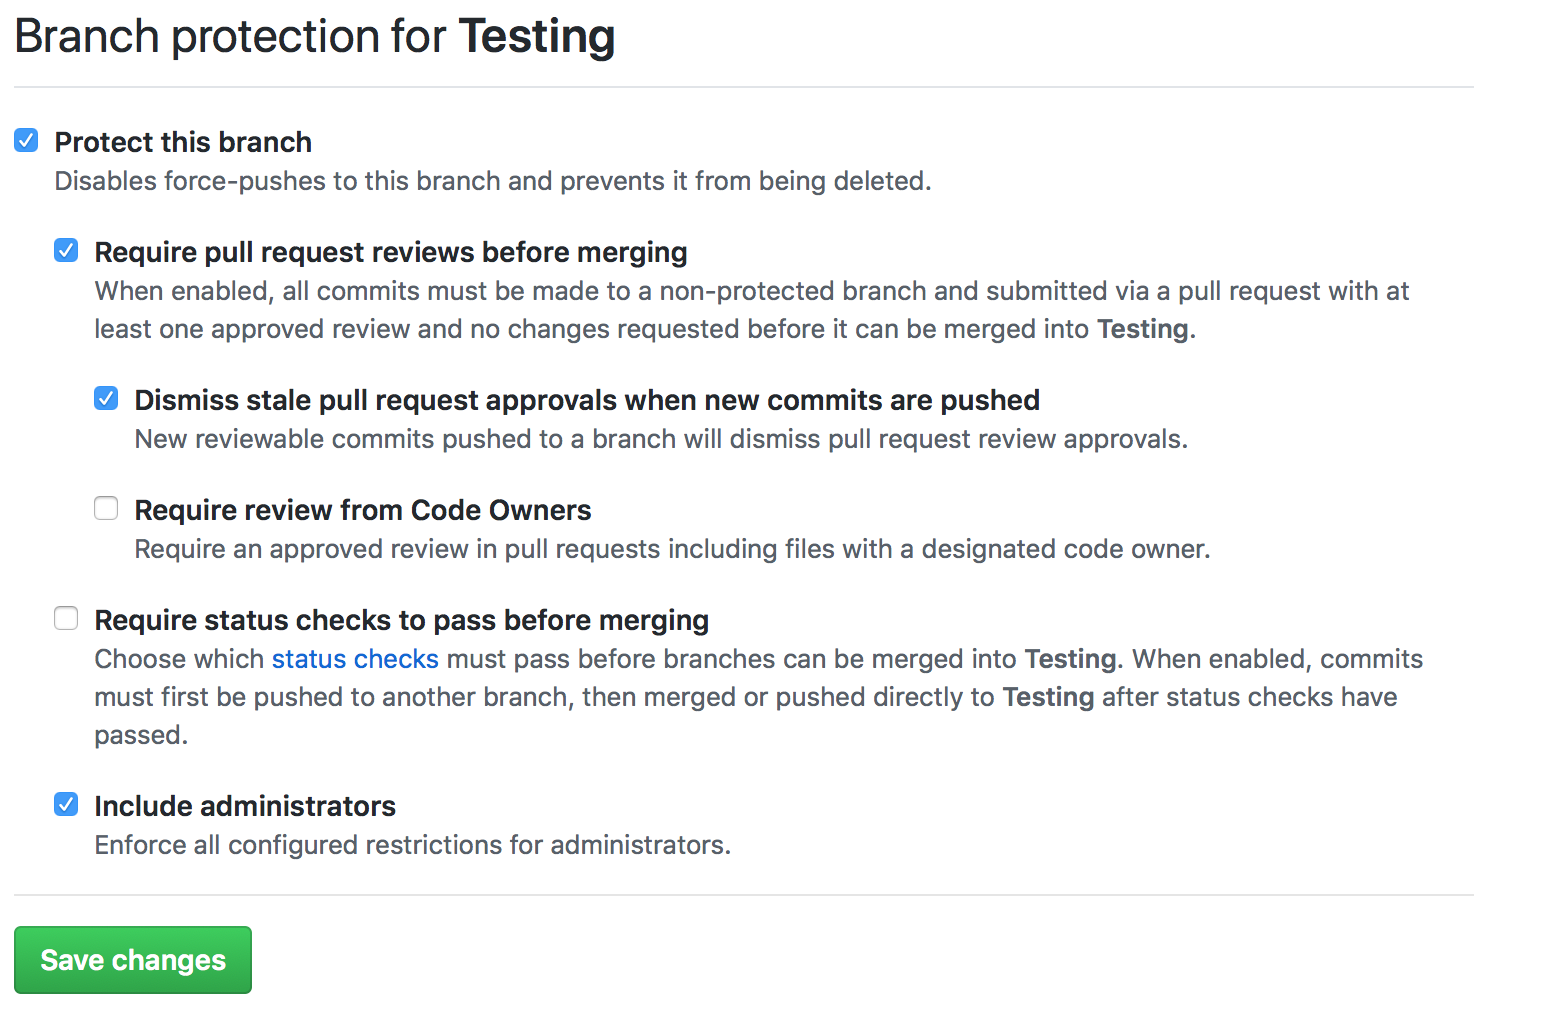
\includegraphics[width=0.5\textwidth]{images/BranchProtectionSetup.png}
	\caption{Overzicht van protectie wat ingesteld is op branch}
	\label{fig:BranchProtectionSetup}
	\end{figure}
	
	\subsection{Testing}
	De Testing-branch zal gebruikt worden om nieuwe functionaliteit die ontwikkeld zijn in de development branch te testen. Wanneer de functionaliteit in de testing branch geaccepteerd wordt, zal deze worden doorgezet naar de master branch zodat de verbeteringen en/of nieuwe wijzigingen beschikbaar zijn voor alle gebruikers op de productie omgeving
	De Testing-branch heeft dezelfde setup als de Master-branch. Dit wilt zeggen dat het op deze branch ook niet mogelijk is om rechtstreeks code te committen.
	\subsection{Development}
	
	De Development-branch bevat nieuwe functionaliteit of verbeteringen wat ontwikkeld zijn. Deze branch is vrij toegangkelijk voor de ontwikkelaar om eventueel kleine(re) verbeteringen door te voeren.	
	Het is als nog de bedoeling dat nieuwe functionaliteit niet rechtstreeks op deze branch wordt gecommit. Mocht een ontwikkelaar nieuwe functionaliteit of grotere verbeteringen willen ontwikkelen, kan hiervoor een zogenaamde Feature-branch worden aangemaakt. Meer informatie hierover is in de volgende alinea te lezen
	
	\subsection{Features}
	De Features-branch is geen branch die direct aangemaakt is op Github. Dit komt doordat "Features" een overkoepelende term is. Wanneer een ontwikkelaar nieuwe functionaliteit of verbeteringen wilt ontwikkelen, dan zal hiervoor een nieuwe branch moeten worden aangemaakt, bijvoorbeeld "Dev-exampleFeature". Aan de hand van de prefix "Dev-" weet iedereen dat dit een branch betreft waar nieuwe functionaliteit of verbeteringen op worden ontwikkeld. Het gedeelte achter de prefix moet dan ook beschrijven aan welke functionaliteit of verbeteringen worden gewerkt.
	
	
	Wanneer de ontwikkelaar het implementeren heeft voltooid, zal dit eerst getest moeten worden op zijn eigen, lokale omgeving. Wanneer die nieuwe functionaliteit werkt met de rest van de ontwikkelde software, kan de ontwikkelaar zijn branch, bijvoorbeeld "Dev-exampleFeature" gaan samenvoegen met de Development-branch. Hiervoor maakt de ontwikkelaar een merge request aan wat ervoor zorgt dat diene nieuwe code wordt samengevoegd op de Development-branch.

	\chapter{Code Style}
Voor de code style worden de standaard code style settings van IntelliJ IDEA gebruikt.
De code style wordt ook gecontroleerd door Codacy, een code analyse tool.
Codacy controleert je Java (en Javascript) codebase op verschillende errors.

\begin{figure}[H]
	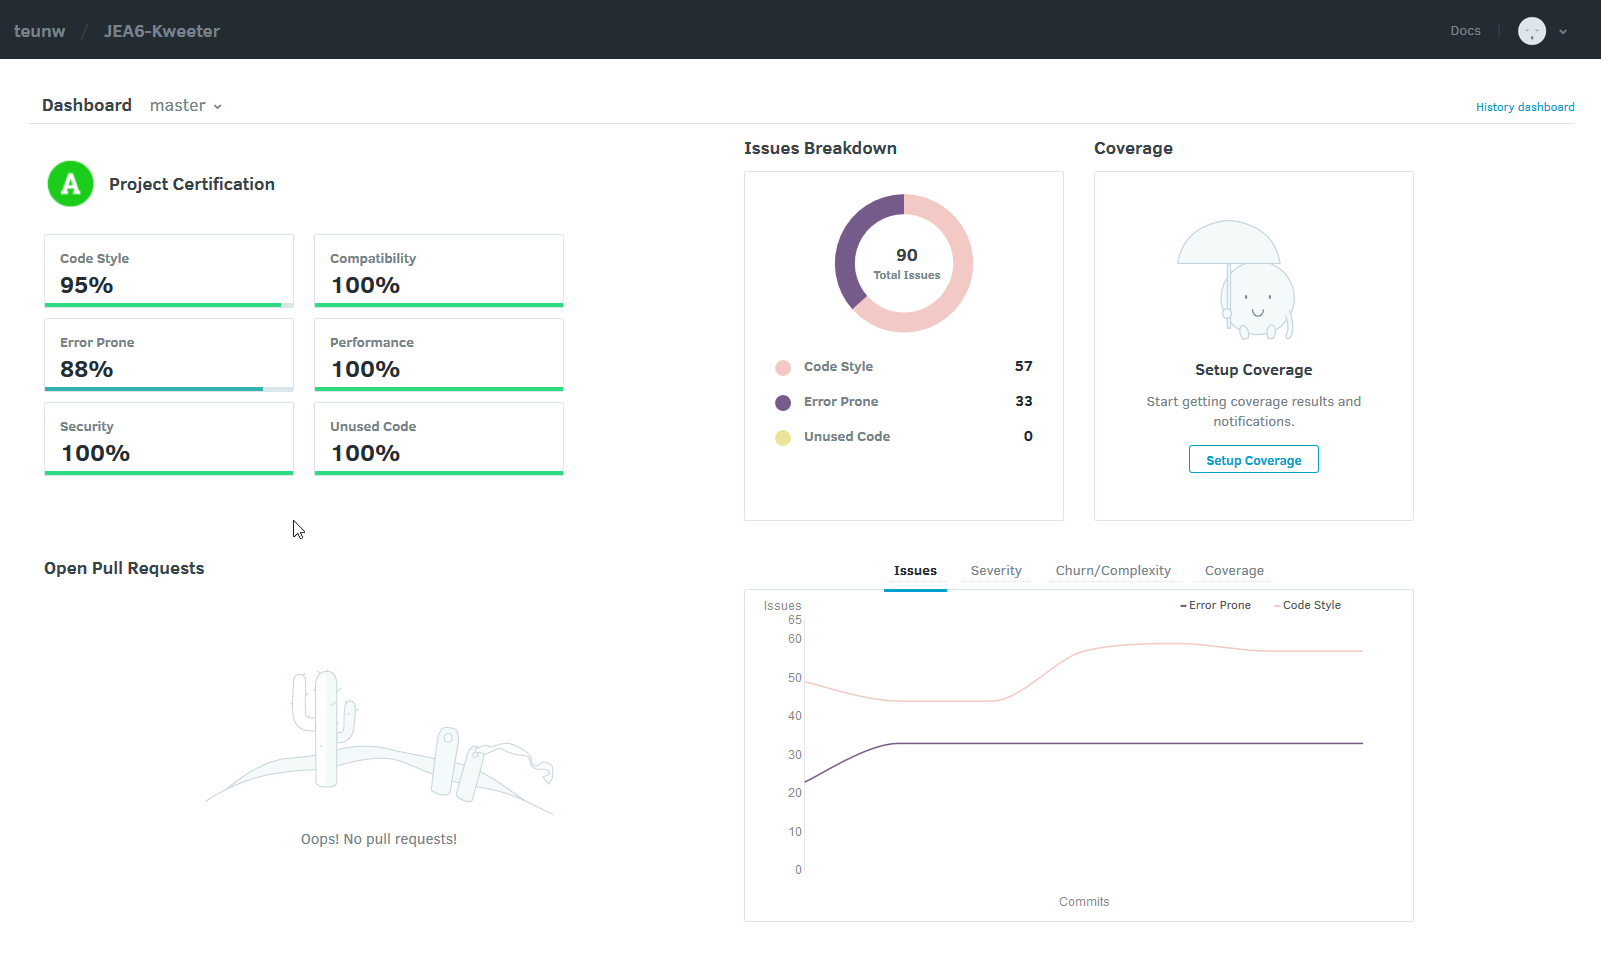
\includegraphics[width=0.75\textwidth]{images/StaticCodeAnalysis.png}
	\caption{Voorbeeld van code analysis door middel van Codacy}
	\label{fig:StaticCodeAnalyses}
\end{figure}

Ook kan er gecontroleerd worden op beveiligingsproblemen in je applicatie, stel dat je bijvoorbeeld SQL-query parameters in je queries hebt staan, dan wordt dat netjes gerapporteerd.
Andere dingen waartegen je beschermt wordt zijn:
\begin{itemize}
	\setlength\itemsep{0em}
	\item Authentication
	\item CSRF aanvallen
	\item File access
	\item SQL Injection
	\item XSS
\end{itemize}

Natuurlijk bied Codacy ook een gedetaileerd overzicht van de verschillende fouten in je code.
\begin{figure}[H]
	\centering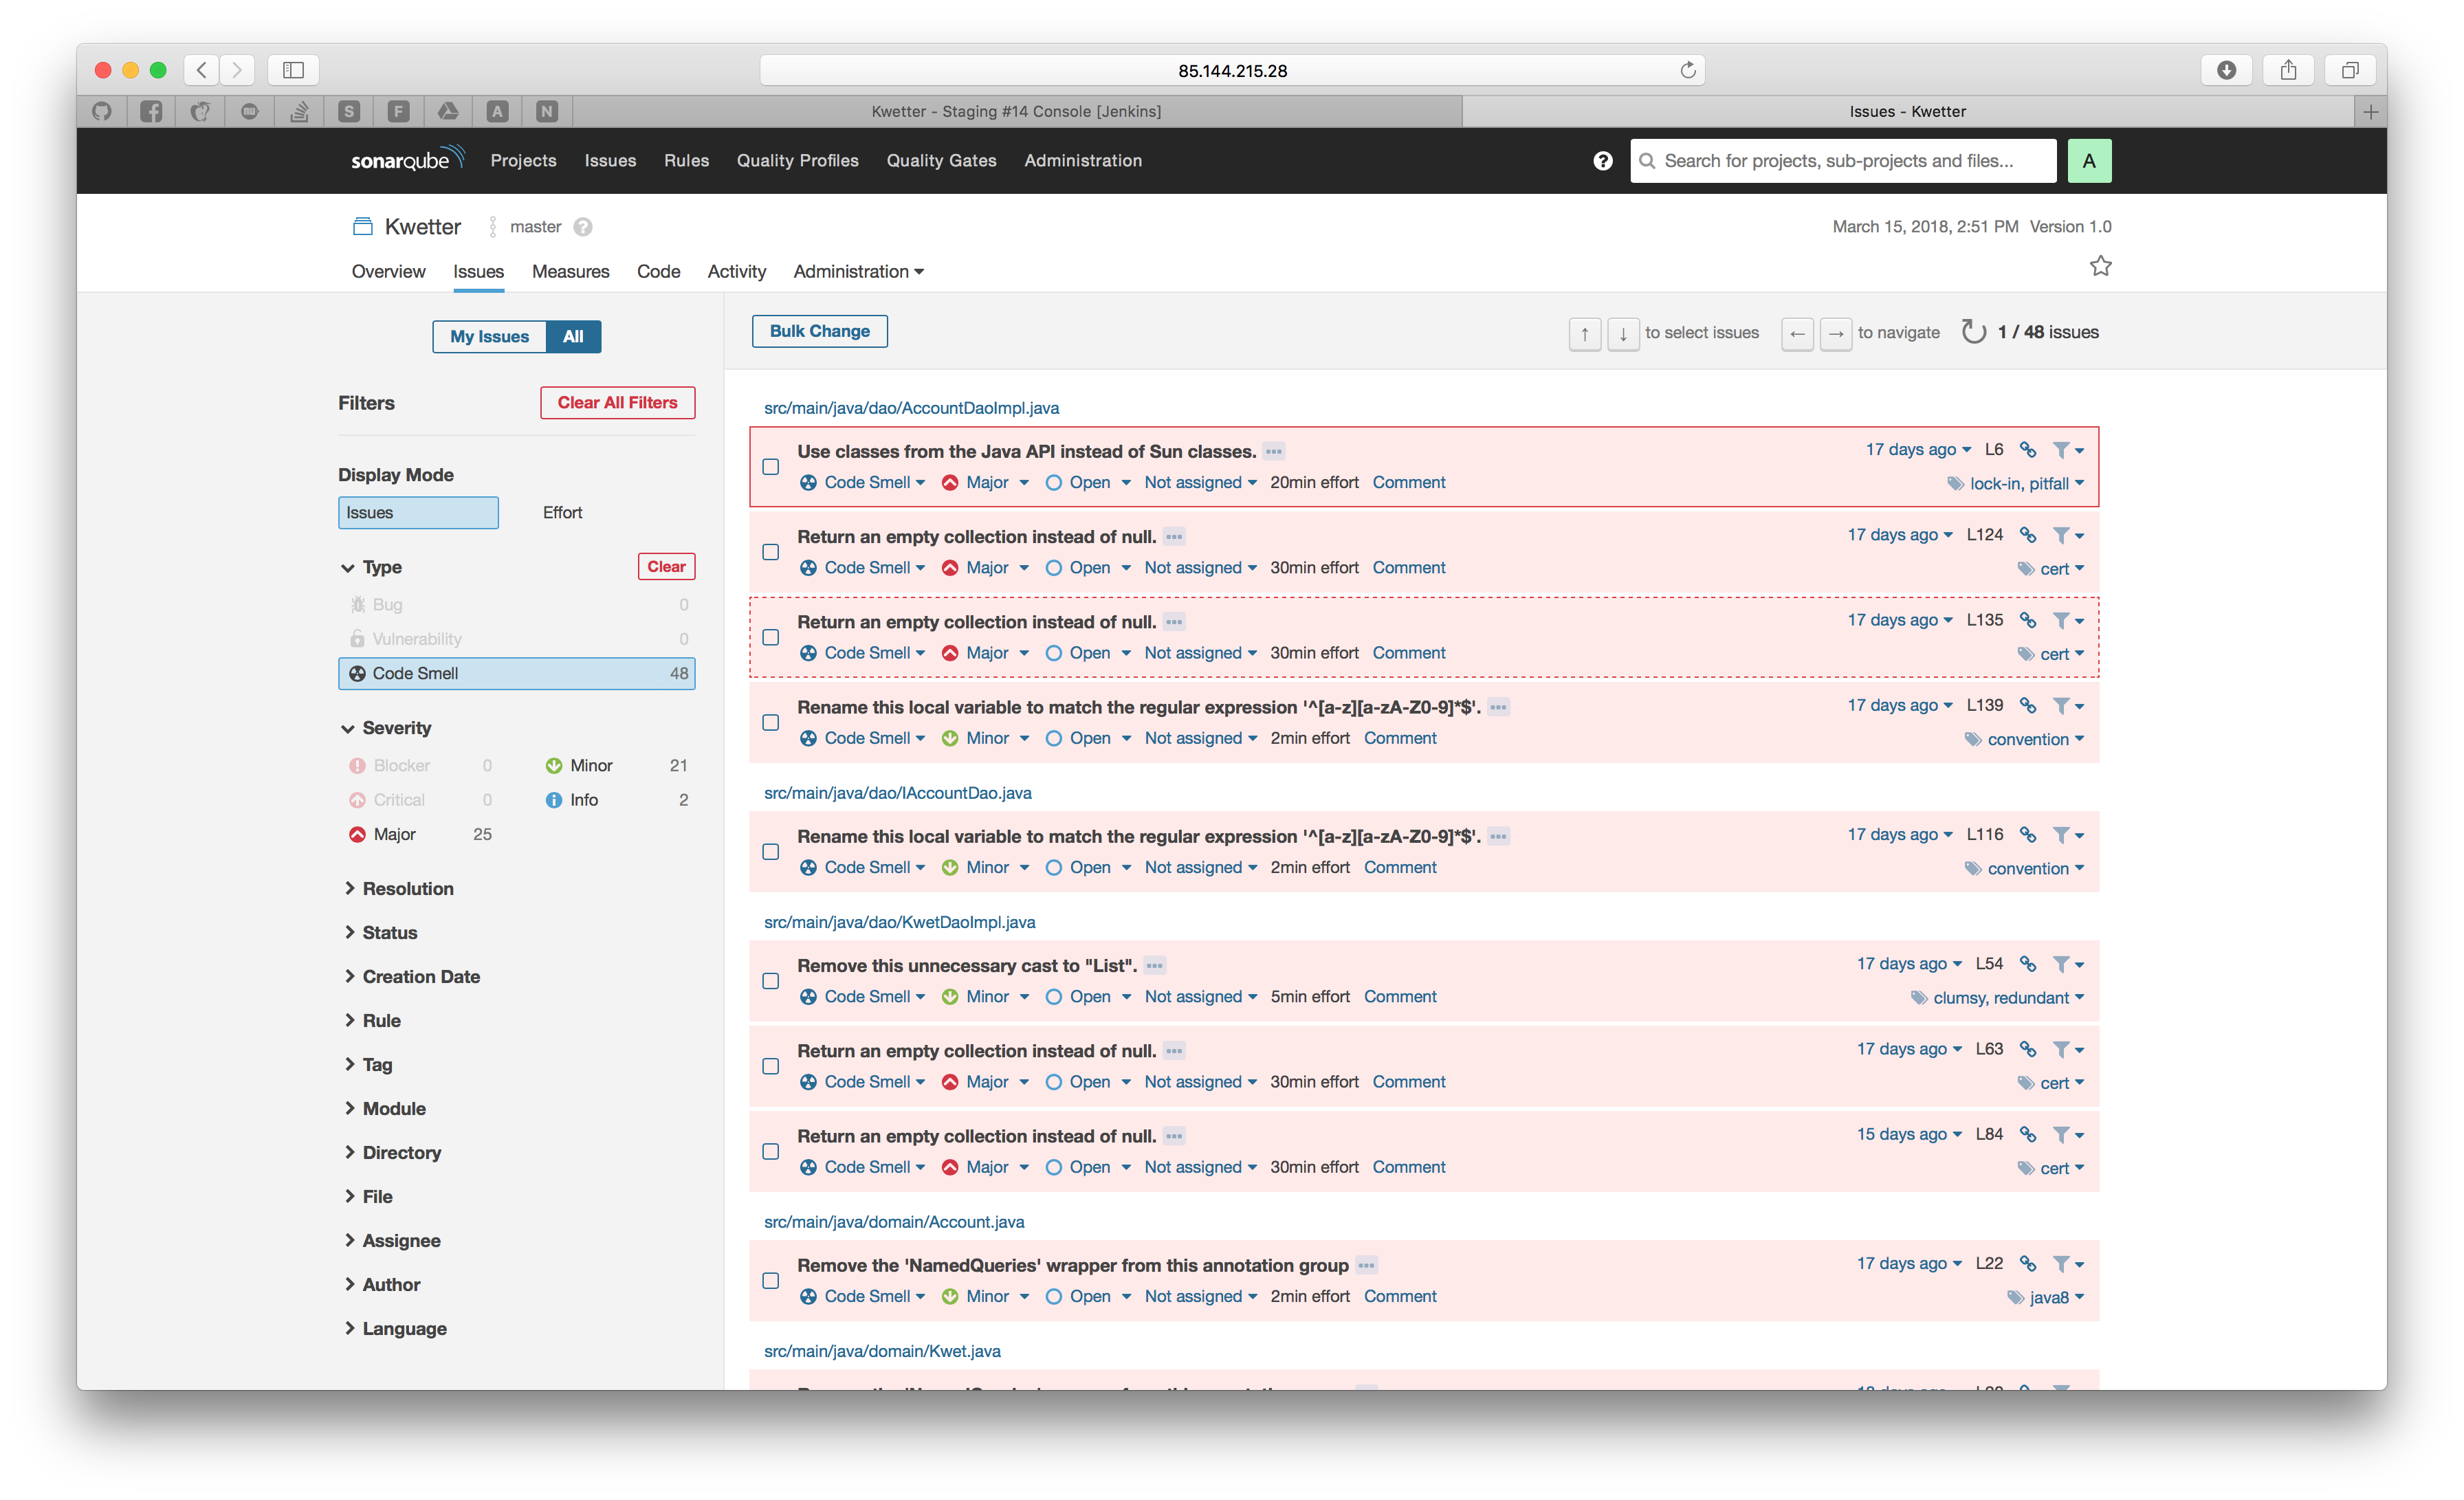
\includegraphics[width=0.5\textwidth]{images/Codacy}
	\caption{Verschillende fouten in een Typescript bestand}
\end{figure}

\section{Release}
Codacy heeft de mogelijkheid om branches individueel te controleren op code.
Hierdoor kan je per branch inzien wat voor cijfer deze krijgen.
Branches worden aan een hoge standaard gehouden, de code moet minimaal een A krijgen om te mogen mergen met de development.
\begin{figure}[H]
	\centering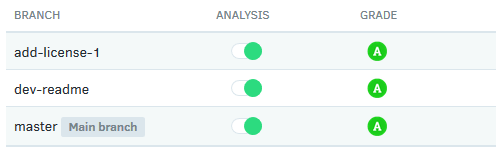
\includegraphics[width=0.55\textwidth]{images/CodacyBranchGrades}
	\caption{Branches en hun cijfer}
\end{figure}
Er is geen infrastructuur om te zorgen dat code met een laag cijfer niet gemerged kan worden, dit is een limitatie van de infrastructuur (dus van Github en Codacy).
Op hotfix branches hoeft niet meteen een controle uitgevoerd te worden, aangezien een hotfix zo snel mogelijk live moet zijn is dit onwenselijk.
Wel zou deze controle uitgevoerd moeten worden nadat de hotfix toegepast is, omdat slechte code in deze branch het mergen van andere zou kunnen hinderen.
De ontwikkelaar is verantwoordelijk voor zijn/haar eigen branch, het is de taak van de ontwikkelaar om een slecht cijfer te repareren.

	
	\chapter{Continuous Integration}
Continuous is geregeld door TravisCI, voor open source projecten is TravisCI gratis te gebruiken.
Omdat het project met Gradle is gebouwd is het makkelijk om CI ondersteuning toe te voegen aan de backend.
Het commando "gradle test" draait alle tests in het project, als er iets fout gaat is dit ook meteen in Github zichtbaar.
\linebreak
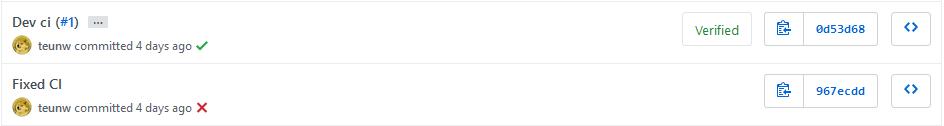
\includegraphics[width=\textwidth]{images/TravisCI.png}
	\chapter{Testing}
	\chapter{Versioning}
Door gebruik te maken van versioning kan het voor een ontwikkelaar duidelijk zijn in welke versie van de software een eventueel probleem is aangetroffen. 
Een manier om versioning toe te passen is door gebruik te maken van Semantic Versioning (versie 2.0.0).
Meer informatie en de volledige specificatie ven Semantic Versioning is beschikbaar op hun website: \url{https://semver.org}

Bij Semantic Versioning is een versienummer opgebouwd uit drie verschillende delen. Namelijk:
\begin{itemize}
	\item Major
	\item Minor
	\item Patch
\end{itemize}

\section{Major}
Het eerste getal van het versie nummer geeft de versie van de software aan. Dit getal begint meestal bij 1, maar in sommige gevallen kan ook versie 0 voorkomen. In deze gevallen geeft de 0 aan dat de software nog in ontwikkeling is, en dat de software nog niet als "stable" gezien kan worden.
Wanneer het major nummer van de versie veranderd, geeft dit meestal aan dat er wijzigingen in de API zijn gedaan die niet meer compatible zijn met een vorige versie. Zo kan de data die naar een endpoint gestuurd wordt bijvoorbeeld op een andere manier worden terug gegeven.

\section{Minor}
Het tweede getal in het versienummer geeft aan welke wijziging zijn toegevoegd aan het huidige software pakket. Wijzigingen die ervoor zorgen dat het minor getal toeneemt, is meestal nieuwe functionaliteit wat beschikbaar wordt gesteld. Een vereiste van deze functionaliteit is dat deze compatible is met de huidige implementatie van de software.
Wanneer een of meerdere functie's niet meer ondersteund worden, moet dit volgens de Semantic Versioning specificatie ook worden weergegeven in het minor nummer van de versie.

\section{Patch}
Wanneer in de huidige versie van de software een fout wordt ontdek en dit verholpen moet worden, een zogenaamde "bugfix". Deze bugfix kan ook worden weergegeven in het versienummer van de software. Dit gebeurt aan de hand van het derde nummer: het patch nummer. Het is vanzelfsprekend dat de huidige functionaliteit niet veranderd mag worden. Mocht dit wel het geval zijn, dan is het ook vereist dat het major of minor nummer van de versie aangepast wordt.

\section{Overige Informatie}
Bij de opbouw van het versie nummer is het niet toegestaan om een nummer te laten beginnen met 0 (bv. 1.01.0 is niet toegestaan). Een uitzondering hierop is de opbouw van het versie nummer wanneer de software nog in ontwikkeling is zoals beschreven in \textit{5.1 Major}.

Wanneer ervoor gekozen wordt om een pre-release versie van de software beschikbaar te stellen, kan dit tevens worden weergegeven in het versie nummer. Dit gebeurd door de versie van de pre-release door middel van een koppelteken te plaatsen achter het daadwerkelijke versie nummer van de software. Een aantal voorbeelden hiervan zijn: 1.0.0-alpha, 1.0.0-alpha.1, 1.0.0-0.3.7

Eventuele build metadata mag tevens worden weergegeven in het versie nummer. Dit wordt gebruikelijk direct na het patch nummer of de pre-release versie weergegeven met behulp van het koppelteken +.
	\chapter{Continuous Delivery}
Met TravisCI kun je ook continuous delivery regelen, op de Travis worden verschillende providers genoemd.

\begin{figure}[H]
	\centering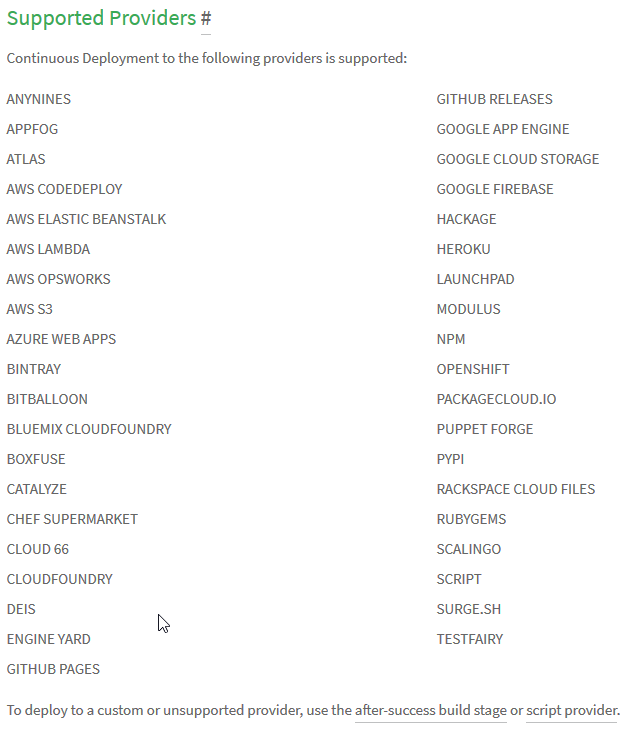
\includegraphics[width=0.35\textwidth]{images/TravisCICDProviders}
	\caption{Providers met support in TravisCI}
\end{figure}
Het deployen van applicaties gebeurt ook via de .travis.yml.
Omdat de .travis.yml file publiekelijk toegangkelijk is, is er ook de mogelijkheid om de wachtwoorden van verschillende services encrypted in de file te zetten.
Deze encryptie moet ervoor zorgen dat anderen niet zomaar op jouw account acties kunnen uitvoeren.

\section{Deployment}
Deployment wordt gergeld via eigen servers op het infralab van Fontys.
Omdat de applicatie op JavaEE gebouwd is moet de applicatie gedeployed worden op een applicatieserver.
Voor deze applicatieserver is Wildfly gekozen, een applicatieserver voor JBOSS JavaEE based applicaties.
Met Wildfly kunnen applicaties gedeployed worden met een console commando.
\end{document}